% Why the simulated and the observed momentum enhancement are not the
% same projection. The point is the triangle at the impact site, so the
% binary geometry is demoted to a small inset.
% Compile from `docs/preprint`:  lualatex sekil/projeksiyon.tex
\documentclass[border=3pt,tikz]{standalone}
\usepackage{amsmath}
\usepackage[outline]{contour}
\usetikzlibrary{angles,quotes,calc,arrows.meta}
\contourlength{1.0pt}
\tikzset{>=latex}

\colorlet{ink}{black!82}
\colorlet{orbcol}{blue!55!cyan!75!black}
\colorlet{impcol}{red!75!black}
\colorlet{ejcol}{orange!88!black}
\colorlet{gh}{black!42}

\begin{document}
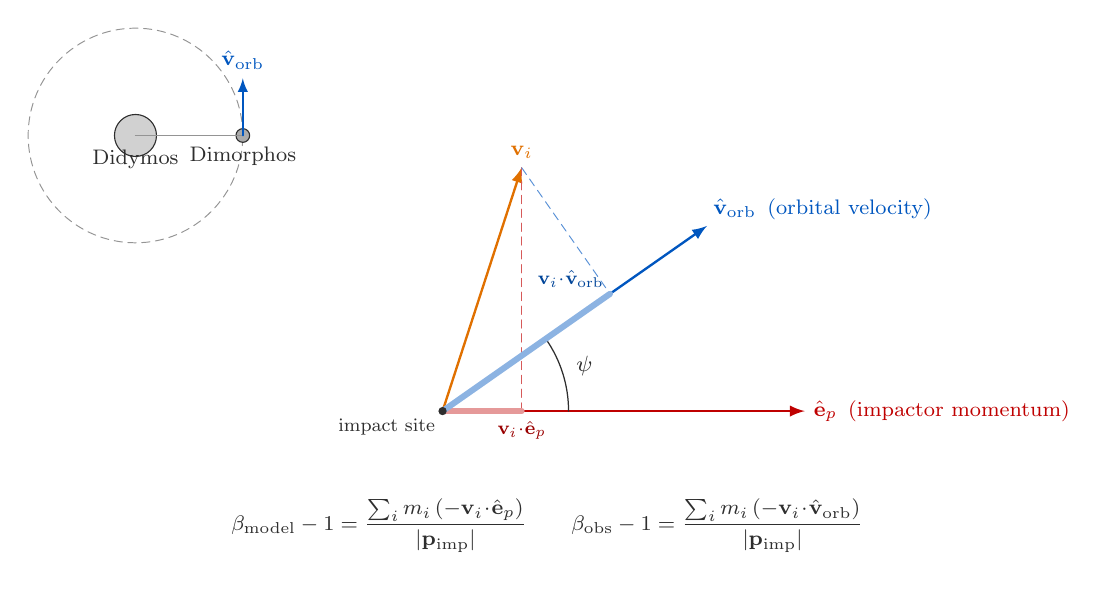
\begin{tikzpicture}[
    font=\footnotesize, line cap=round,
    vec/.style={->, line width=0.85pt},
    thin_/.style={line width=0.35pt, draw=gh},
  ]

\coordinate (O) at (0,0);

% --- the two reference directions -------------------------------------
\coordinate (P) at (4.6,0);                 % impactor momentum
\coordinate (V) at (35:4.1);                % orbital velocity
\draw[vec, impcol] (O) -- (P)
      node[anchor=west, impcol, scale=0.95, inner sep=3pt]
      {$\hat{\mathbf e}_p$\, (impactor momentum)};
\draw[vec, orbcol] (O) -- (V)
      node[anchor=south west, orbcol, scale=0.95, inner sep=2pt]
      {$\hat{\mathbf v}_{\rm orb}$\, (orbital velocity)};

% `P--O--V`, not the reverse: `angle` sweeps counter-clockwise, and the
% other order marks the reflex angle.
\pic[draw=ink, line width=0.45pt, angle radius=16mm, angle eccentricity=1.18,
     "$\psi$"{ink, scale=1.0}] {angle = P--O--V};

% --- one ejecta parcel -------------------------------------------------
\coordinate (E) at (72:3.25);
\draw[vec, ejcol] (O) -- (E)
      node[anchor=south, ejcol, scale=0.95, inner sep=3pt]
      {$\mathbf v_i$};

% --- its two projections ----------------------------------------------
\coordinate (Ep) at ($(O)!(E)!(P)$);
\coordinate (Ev) at ($(O)!(E)!(V)$);

\draw[thin_, densely dashed, impcol!65] (E) -- (Ep);
\draw[thin_, densely dashed, orbcol!65] (E) -- (Ev);
\draw[line width=2.2pt, impcol!40] (O) -- (Ep);
\draw[line width=2.2pt, orbcol!45] (O) -- (Ev);

\node[impcol!80!black, scale=0.85, anchor=north, inner sep=4pt] at (Ep)
     {$\mathbf v_i\!\cdot\!\hat{\mathbf e}_p$};
\node[orbcol!80!black, scale=0.85, anchor=south east, inner sep=2.5pt] at (Ev)
     {\contour{white}{$\mathbf v_i\!\cdot\!\hat{\mathbf v}_{\rm orb}$}};

\fill[ink] (O) circle (1.5pt);
\node[ink, scale=0.85, anchor=north east, inner sep=3pt] at (O) {impact site};

% --- the binary, as an inset: it only fixes where v_orb points ---------
\begin{scope}[shift={(-3.9,3.5)}, scale=0.58]
  \coordinate (K) at (0,0);
  \coordinate (D) at (2.35,0);
  \draw[thin_, densely dashed] (K) circle (2.35);
  \fill[ink!22, draw=ink, line width=0.4pt] (K) circle (0.46);
  \fill[ink!40, draw=ink, line width=0.4pt] (D) circle (0.15);
  \draw[thin_] (K) -- (D);
  \draw[->, orbcol, line width=0.7pt] (D) -- ++(0,1.25);
  \node[ink, scale=0.95, below=2pt] at (K) {Didymos};
  \node[ink, scale=0.95, anchor=north, inner sep=4pt] at (D) {Dimorphos};
  \node[orbcol, scale=0.95, anchor=south] at ($(D)+(0,1.25)$)
       {$\hat{\mathbf v}_{\rm orb}$};
\end{scope}

% --- the statement ----------------------------------------------------
\node[ink, scale=0.95, anchor=north west, align=left] at (-2.8,-1.0)
  {$\displaystyle \beta_{\rm model}-1
     =\frac{\sum_i m_i\,(-\mathbf v_i\!\cdot\!\hat{\mathbf e}_p)}
           {|\mathbf p_{\rm imp}|}
   \qquad
   \beta_{\rm obs}-1
     =\frac{\sum_i m_i\,(-\mathbf v_i\!\cdot\!\hat{\mathbf v}_{\rm orb})}
           {|\mathbf p_{\rm imp}|}$};

\end{tikzpicture}
\end{document}
